%*********************************************************************
%	CHAPTER 5 - EXPERIMENTAL PROCEDURE
%*********************************************************************
\chapter{Experimental procedure}
\label{ch:experiments}
%---------------------------------------------------------------------

%=====================================================================
\section{Experimental setup}
\label{sec:ch5.setup}
%=====================================================================
% Rig, tank, lighting, turbidity control, ground truth measurement




%=====================================================================
\section{Experiment 1: Stereo calibration in air and underwater}
\label{sec:ch5.exp1_calibration}
%=====================================================================
% Calibration tests (in air vs underwater)
Initial underwater tests were done into the sun, not at full quality (oops).
This resulted in minimal detection and an initial default detection of ...


\subsection{Frame selection and blur checking}
Frame selection and extraction is done via a extract\_Stereo\_frames.py. 
The frames can be manually selected and labelled through a viewier, or autoselected at
specified step intervals. It also allows for the storing o....

XXX..py does analysis on the selected frames, looking at x,y,z metrics to ensure good??

There were concerns regarding the YUYV blur and shutter time.This allows for good comparison 
between the two. Briefly explain what makes one blurry %DOI 10.1109/SYSMART.2016.7894491







\subsection{Calibration}
The Calibration for determining the systems intrinsics and extrinsics were completed
using calibration.py. This allowed for quick iteration of openCV detector configurations. For this
comparison, tags detected is the metric. Outputs a png with the noted detectrions. See image below.
add in the DetectedTags.png here
\begin{figure}[H]
    \centering
    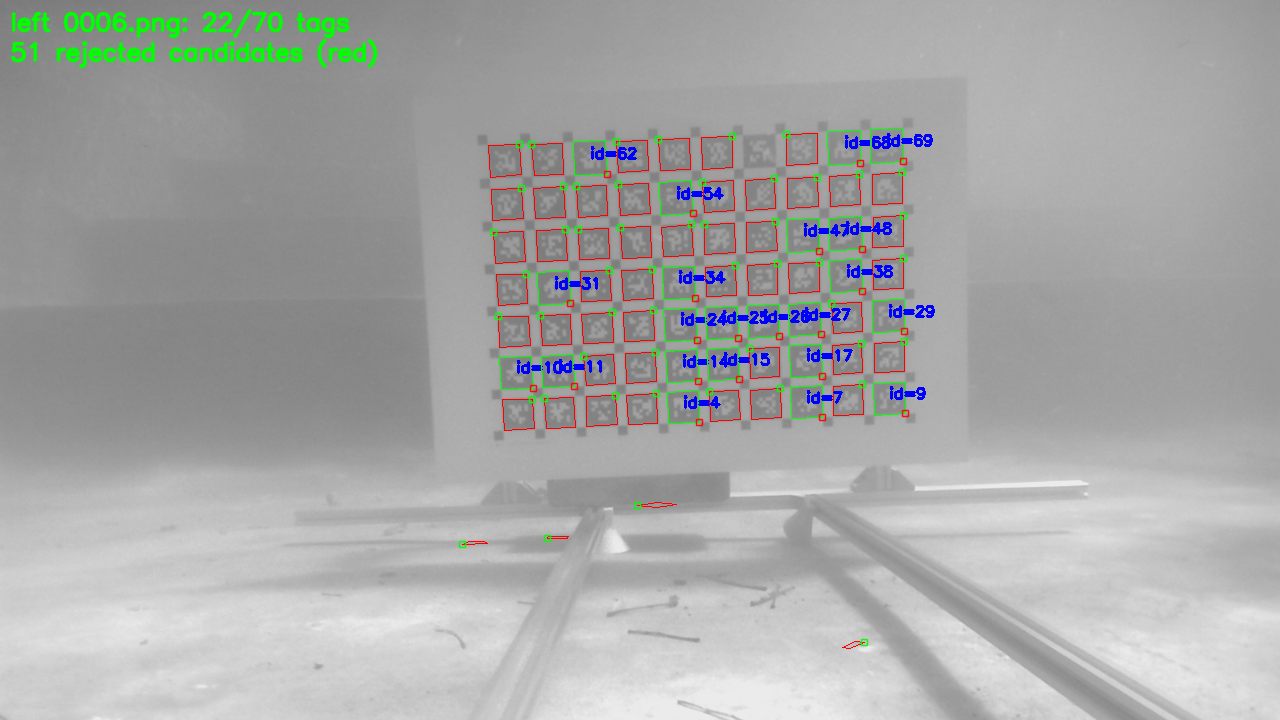
\includegraphics[width=0.8\textwidth]{figs/Ch5/DetectedTags.png}
    % CLAUDE: caption below is still the template placeholder; \cite{key} prints [?]. Replace with your own caption.
    \caption[Short caption for the List of Figures.]{\textbf{Bold lead-in sentence.}
        Longer explanation of what the reader is looking at. Taken from \cite{key}.}
    \label{fig:ch5.detectedtags}
\end{figure}


\subsubsection{Optimising for Detection}
% Mention how to optimise through varying openCV parameters
% Mention metrics for what is good, explained in the theoretical development
%=====================================================================


Comparing channel selection , channel gain mixing


MAINLY TWEAKED OPENCV for improved detections.

TESTING CLAHE AND IMPROVING DETECTIONS WITHOUT MESSING UP ACCURACY
CONCERNS OVER CLAHE NON-LINEAR MAPPING 
HARD BECAUSE IT GETS HAZY, FLOATING DEBRIS IN THE WAY (HAVE FIGURE REFERENCEING CLOSE UP AD DIFFERENT DISTANCES)


SAFE FOR BOTH 
PER-PIXEL, SPATIALLY UNIFORM TRANSFORMS : GAMM, CONTRAST STRERTCH, PER-CHANNEL GAIN CHANNEL MIXING, CHANNEL SELECTION
SIMPLE DEHAZING: I=J.t+b.(L-T)... something about dehazing not moving a corner
Symmetric linear filters: Gaussian bluer, unsharm mask
UPSCALING?


Metrics:
-  Tag detection vs distance + false ids
- Triagnulated tag-size error in mm (of stereo reconstruction) at same distance? or different distanec?
         - use frames not used in calibrate (Ems board across different distances)
- RMS Reprojection error on the common set of tags. Better detector gets ones with noiser corners, makes error worse punishment for good work
        - COncenrs  (internal, measures how well model fits data, not accurate result)
- OpenCV uncertainty values
    

- false-ids.
Compare RMS error across ONLY those matching tags across all. NB to ensure not loosing accuracy across any of the enhancements

The method relies on high gradients

Detection count:
First: Standard OpenCV setup, full colour
Second: Comparing the Gray, RGB colours 
Third: 

WRITEUP:
% Intro to the colour comparison
The first part was choice was to compare the how aprilgrid detection works for the different channels. OpenCV's apriltag
detection only takes a single colour input channel Due to underwater different absorption, the tag's contrast differes depending
on colour channel The analyse this comparison, five inputs: grayscale converted using? , the camera's JPEG luma (Y), and the red, 
green and blue channels. 

Each run was done using the OpenCV calibration defaults, using the same set of calibration frames. Each run is judged on tag detection amount
(as a fraction of the 70 board frames),  false detection rate, and the RMS reprojection error over the images that are common to all the runs.


% analysing the coloour comparioson
Grayscale and Y gave the same results, a mean recall of X and Y RMS for the ledt camera. This is expected as the JPEG luma uses the same RBG weigths as
grayscale. Red and green ach found X less, with Blue the clear worse with X and Y error. Likely blue half resoluition (research).

\begin{figure}[htbp]
    \centering
    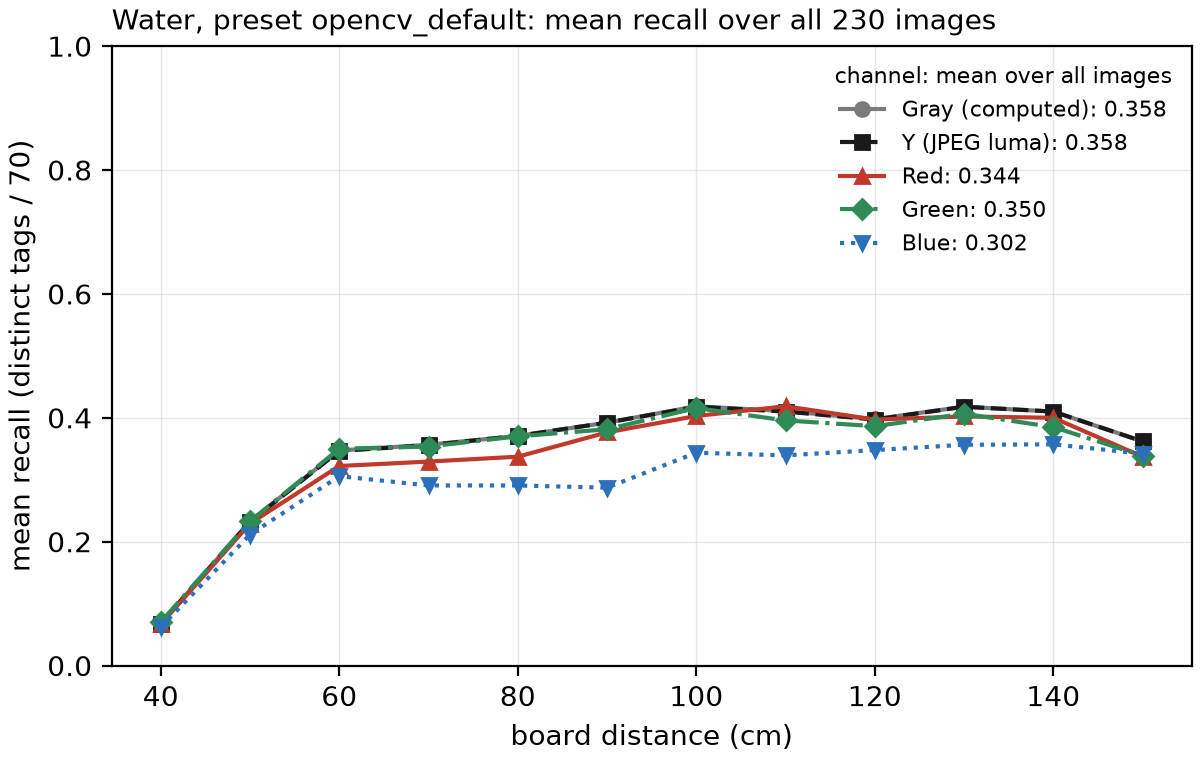
\includegraphics[width=0.8\textwidth]{../results/analysis/channel_selection_opencv_default/fig_recall_mean.png}
    \caption[short caption]{\textbf{Lead-in.} Description.}
    \label{fig:ch1.name}
\end{figure}

% Joining the different detections for maximum number of detections

It was noted by (HOW DID I DETECT THIS) that some of the tags being detected by the grayscale
did not fully overlap with th ose detected byu tohers (i.e. red got some grey did not). This is shwon in 
figure X below
TO maximise tag detection, they were run seperately and merged to maximise usable images. 

\begin{figure}[htbp]
    \centering
    \includegraphics[width=0.8\textwidth]{../results/analysis/channel_selection_opencv_defualt/gih_channel_overlap_L3.png}
    \caption[short caption]{\textbf{Lead-in.} Description.}
    \label{fig:ch1.name}
\end{figure}



% OpenCV parameter adjustments, what, why, ,how (educated guess, followed by paramtere sweep), improved detection results
The next thing to do was to play / adjust opencv's calibration method's parameters. A parameter sweep was 


\begin{table}[H]
    \centering
    \caption[ArUco detector parameters.]{\textbf{ArUco detector parameters.} The detector settings exposed through \texttt{detector\_presets.json}, their defaults, and the conditions under which each is adjusted.}
    \begin{tabularx}{\textwidth}{>{\raggedright\arraybackslash}m{3.6cm}>{\raggedright\arraybackslash}m{1.2cm}>{\raggedright\arraybackslash}X>{\raggedright\arraybackslash}X}
    \toprule[2.25pt]
    \textbf{Setting} & \textbf{Default} & \textbf{What it does} & \textbf{When to set it} \\
    \midrule[1pt]
    \texttt{adaptiveThreshWinSizeMin} & 3 & Smallest neighbourhood (px) for computing the local threshold. & Increase for noisy images. \\
    \texttt{adaptiveThreshWinSizeMax} & 23 & Largest neighbourhood. & Raise for large lighting area variations, or close to the camera. \\
    \texttt{adaptiveThreshWinSizeStep} & 10 & Step between window sizes; each size is a separate thresholding pass. & Lower for more passes, at the cost of speed. \\
    \texttt{adaptiveThreshConstant} & 7 & Offset subtracted from the local mean before comparing. & Lower for low-contrast, hazy images. \\
    \midrule
    \texttt{minMarkerPerimeterRate} & 0.03 & Minimum tag perimeter as a fraction of the larger image dimension. & Lower to detect small or distant tags. \\
    \texttt{maxMarkerPerimeterRate} & 4.0 & Maximum tag perimeter. & Rarely needs changing. \\
    \texttt{polygonalApproxAccuracyRate} & 0.003 & How far a contour may deviate from a perfect square. & Raise for distortion. \\
    \bottomrule[2.25pt]
    \end{tabularx}
    \label{table:ch4.detectorparams}
\end{table}


% Which I adjusted and why

% Reslts of parameter sweep.




% ACCURACY CHECK, OVERLAPPING

\section{Experiment 2: Reconstruction of known objects}
\label{sec:ch5.exp2_knownobjects}
%=====================================================================


%=====================================================================
\section{Experiment 3: Upward-facing reconstruction of a sea ice model}
\label{sec:ch5.exp3_seaice}
%=====================================================================

\subsection{Colour choice}
Blue to represent 

% https://en.wikisource.org/wiki/Page:The_Botany_of_the_Antarctic_Voyage.djvu/539
% https://archive.org/details/botanyofantarcti01hook

"Pancake-Ice a pale ochreous colour."
"uniformly stained brown"

Ito et al. (2025), JGR: Oceans. https://doi.org/10.1029/2024JC021689
"ice turned clearly ochre during a phytoplankton bloom"

\url{https://doi.pangaea.de/10.1594/PANGAEA.870704?format=html#download}
"Lighting conditions"




\subsection{Material choice}

\subsection{Manufacturing process}
- DIY foam cutting, live cad model, Lidar scanned.
\subsection{Physical properties}
-Holes (few mm to 1 mm wide to miimic drainage channels)
- Overhangs wheree the lip hides surface from one camera- Step discontinuities
- A resolution strip
- Small ride or keel


%*********************************************************************
% END
%*********************************************************************
